\documentclass[a4paper,fleqn,longmktitle]{cas-sc}

\usepackage[numbers,sort&compress]{natbib}
\usepackage{amsmath}
\usepackage{amssymb}
\usepackage{graphicx}
\usepackage{booktabs}
\usepackage{multirow}
\usepackage{array}
\usepackage{url}

\makeatletter
\AtBeginDocument{%
  \@ifundefined{@abspage@last}{}{\xdef\lastpage{\@abspage@last}}%
}
\makeatother

\newcommand{\placeholderfigure}[2]{%
  \begin{figure*}[t]
    \centering
    \fbox{%
      \parbox[c][45mm][c]{0.92\textwidth}{%
        \centering
        \textbf{Placeholder figure}\\[4pt]
        #1
      }%
    }
    \caption{#2}
  \end{figure*}
}

\begin{document}
\let\WriteBookmarks\relax
\def\floatpagepagefraction{1}
\def\textpagefraction{.001}

\shorttitle{AutoArchival for Historical Text Spotting}
\shortauthors{L. Liang et al.}

\title[mode=title]{AutoArchival: LLM-Guided Architecture Search\\for Vertical Mongolian-Chinese Historical Text Spotting}

\author[1]{Lanying Liang}
\credit{Conceptualization, Data Curation, Writing -- Original Draft}

\author[2]{Yuefeng Liu}
\cormark[1]
\ead{liuyuefeng@imust.edu.cn}
\credit{Methodology, Software, Validation, Writing -- Review \& Editing, Supervision}

\author[3]{Jianjun Zhao}
\ead{zhao@ait.kyushu-u.ac.jp}
\credit{Writing -- Review \& Editing, Supervision}

\affiliation[1]{organization={Archives, Inner Mongolia University of Science and Technology},
  city={Baotou},
  postcode={014010},
  state={Inner Mongolia},
  country={China}}

\affiliation[2]{organization={School of Artificial Intelligence and Data Science (School of Cyber Security), Inner Mongolia University of Science and Technology},
  city={Baotou},
  postcode={014010},
  state={Inner Mongolia},
  country={China}}

\affiliation[3]{organization={Faculty of Information Science and Electrical Engineering, Kyushu University},
  city={Fukuoka},
  country={Japan}}

\cortext[1]{Corresponding author.}

\begin{abstract}
Joint text detection and recognition in Mongolian-Chinese historical archives remains challenging because of extreme geometric variations, vertical text layouts, and arbitrary physical degradation. Most existing scene text systems are designed either for horizontal detection or for end-to-end text spotting in natural scenes, often failing to adapt to historical archival morphologies without deep manual architectural redesign. In this work, we present AutoArchival, a budget-constrained LLM-guided architecture search framework for end-to-end historical document text spotting. By establishing a fixed-budget evolutionary pipeline bounded by strict computational limitations, the autonomous agent iteratively mutates a baseline end-to-end spotting network at the code level, autonomously adapting convolutional receptive fields, attention mechanisms, and feature pyramid topologies to maximize end-to-end spotting performance. We rigorously evaluate the autonomously discovered network on standard arbitrary-shape and multi-oriented benchmarks (ICDAR 2015 and Total-Text) and a newly introduced Mongolian-Chinese Historical Archive Dataset (MCAD). Experimental results demonstrate that AutoArchival achieves an end-to-end Hmean of 75.3\% on ICDAR 2015 and 76.8\% on MCAD. The method shows clear advantages over baseline architectures on MCAD and maintains competitive performance on public benchmarks while requiring substantially fewer parameters (14.5M).
\end{abstract}

\begin{highlights}
\item LLM-guided search discovers joint spotting architectures for archival text.
\item A fixed budget constrains code-level architecture search and model growth.
\item Vertical-aware modules improve localization-transcription coupling.
\item Public benchmarks and MCAD evaluate end-to-end spotting performance.
\item Ablations analyze search strategy, module gains, and efficiency trade-offs.
\end{highlights}

\begin{keywords}
Joint text detection and recognition \sep
Large language models \sep
Neural architecture search \sep
Mongolian-Chinese archives \sep
Document analysis
\end{keywords}

\maketitle

\section{Introduction}

The digitization and digital preservation of historical manuscripts are critical for the continuity of cultural heritage \cite{alberti2016labeled,zhong2019publaynet,antonacopoulos2009page,chen2021mmocr}. Among these resources, multilingual archives such as Mongolian-Chinese historical documents present unique challenges for automated analysis \cite{zhang2017mongolian,wei2019traditional}. Traditional Mongolian script is written vertically from left to right, which differs substantially from the horizontal alignment of modern Chinese and English text. Historical pages also suffer from severe degradation, including ink bleed-through, faded characters, arbitrary rotation, and dense noisy backgrounds \cite{gatos2006adaptive,tensmeyer2017document,le2019using}.

Current scene text spotting methods such as Mask TextSpotter v3 and ABCNet v2 achieve strong performance on natural images and horizontally organized text \cite{liao2020mask,liu2021abcnet,baek2019character,wang2019shape,zhu2021fourier,liu2018fots}. However, transplanting these models to long-aspect-ratio vertical scripts often leads to missed detections, fragmented bounding boxes, and weak recognition coupling. Adapting such architectures to a domain with highly directional structure usually requires considerable manual expertise or expensive neural architecture search pipelines \cite{zoph2017neural,ghiasi2019nas,liu2019autodeeplab,lyu2021autotext}.

Recent large language models (LLMs) have shown that they can reason over code, modify deep learning pipelines, and iteratively improve algorithmic systems from execution feedback \cite{brown2020language,wei2022chain,yang2024large,yao2023react}. This creates an opportunity to move beyond rigid reinforcement-learning-based NAS pipelines and toward constrained code-level architecture search. Instead of selecting from a small predefined operation pool, the agent can rewrite editable regions of a PyTorch implementation while the surrounding training and evaluation loop remains fixed.

In this paper, we present AutoArchival, a budget-constrained LLM-guided architecture search framework for joint text detection and recognition in historical documents. AutoArchival initializes a lightweight spotting baseline and instructs an LLM agent to mutate predefined architecture regions under a strict five-minute training budget per candidate. Guided by a joint fitness function and bounded compute, the search process discovers specialized operators such as asymmetric convolutions, vertical attention blocks, and vertical alignment mechanisms tailored to archival degradation and long vertical text chains. The main contributions of this work are summarized below.

\begin{enumerate}
\item We introduce AutoArchival, an LLM-driven code-level architecture search framework targeting joint text detection and recognition in historical Mongolian-Chinese archives.
\item We design a budget-constrained joint fitness criterion that balances detection quality and end-to-end spotting quality while discouraging unnecessary model growth.
\item We validate the discovered architecture on ICDAR 2015, Total-Text, and MCAD, showing strong domain adaptation and favorable efficiency-performance trade-offs.
\end{enumerate}

\begin{figure*}[t]
  \centering
  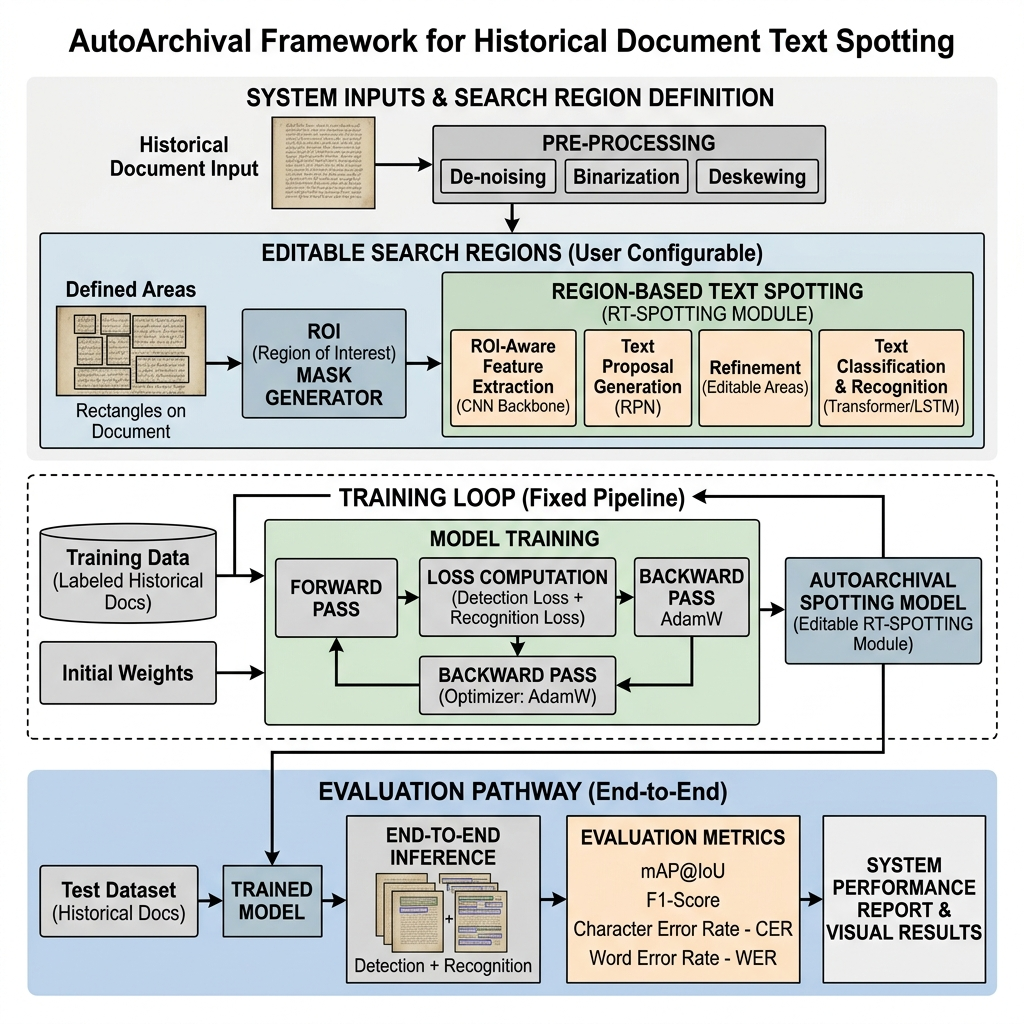
\includegraphics[width=0.95\textwidth]{figures/figure1_pipeline.png}
  \caption{Overview of the AutoArchival framework for joint historical document text spotting, including the editable search regions, fixed training loop, and end-to-end evaluation pathway.}
\end{figure*}

\section{Related Work}

\subsection{Historical Document Analysis}

Text detection in historical documents differs markedly from natural scene text because page images often contain degraded backgrounds, irregular writing surfaces, and mixed structural cues. Public datasets such as DIVA-HisDB and DocBank have supported work on page segmentation and document structure modeling \cite{alberti2017historical,li2020docbank}. However, Mongolian archival documents remain difficult because they contain continuous vertical strokes, bilingual layouts, and strong aspect-ratio asymmetry \cite{gao2021offline,yuan2021novel,zhao2022robust}.

\subsection{Joint Text Detection and Recognition}

End-to-end spotting frameworks couple localization and transcription in a unified network. Representative methods include FOTS, Mask TextSpotter, ABCNet v2, and DeepSolo \cite{liu2018fots,liao2020mask,liu2021abcnet,ye2023deepsolo}. These methods substantially improve over disconnected detector-recognizer pipelines, yet their default inductive biases remain largely symmetric and are mainly optimized for natural scenes rather than vertically organized historical text.

\subsection{Neural Architecture Search and LLM-Based Optimization}

Conventional NAS methods for dense prediction often incur high search cost and rely on fixed search spaces \cite{zoph2017neural,cai2019proxylessnas,liu2019darts,pham2018efficient,he2021automl}. More recent work suggests that LLMs can act as code-level optimizers and iterative research agents \cite{yang2024large,wang2023voyager,yao2023react,shinn2023reflexion}. AutoArchival applies this emerging paradigm to text spotting, where the search target is the coupling between detection and recognition rather than classification accuracy alone.

\section{Proposed Method}

\subsection{Problem Definition}

We formulate archival text spotting as a joint localization-transcription task. Given a historical document image $I$, the model predicts text regions together with a decoded character sequence for each accepted proposal. Detection quality is evaluated independently, but the primary objective is end-to-end spotting, which requires both correct localization and correct transcription.

\subsection{Baseline Joint Architecture}

The search starts from a lightweight baseline that couples feature extraction, proposal generation, region alignment, and sequence decoding. In contrast to conventional OCR pipelines that assume horizontal reading order, our seed model performs vertical RoI alignment so that sequence extraction follows the dominant vertical structure of Mongolian text. The aligned features are decoded with a recurrent recognition head optimized by a connectionist temporal classification (CTC) objective. The recognition vocabulary contains 5,432 symbols spanning simplified Chinese characters, Latin letters, digits, and 35 basic traditional Mongolian letters.

\subsection{Editable Search Space}

Although the search is performed at the code level, it is constrained to predefined editable regions. The LLM agent can rewrite the feature extractor, the region-alignment module, and the recurrent decoder, but it cannot alter the dataset interface, loss definitions, or optimizer schedule. This design keeps the search space expressive while preserving reproducibility and preventing the agent from exploiting non-architectural shortcuts.

\subsection{LLM-Guided Search Loop}

At each iteration, the agent receives the current editable code blocks, validation metrics, runtime logs, and acceptance history. It then proposes a mutated architecture, which is compiled and trained under a 300-second budget. Candidates that fail to compile or diverge during training are rejected. Candidates that satisfy the resource constraints and improve the joint validation objective are retained as new incumbents. Figure~\ref{fig:trajectory} conceptually illustrates this search process.

\begin{figure*}[t]
  \centering
  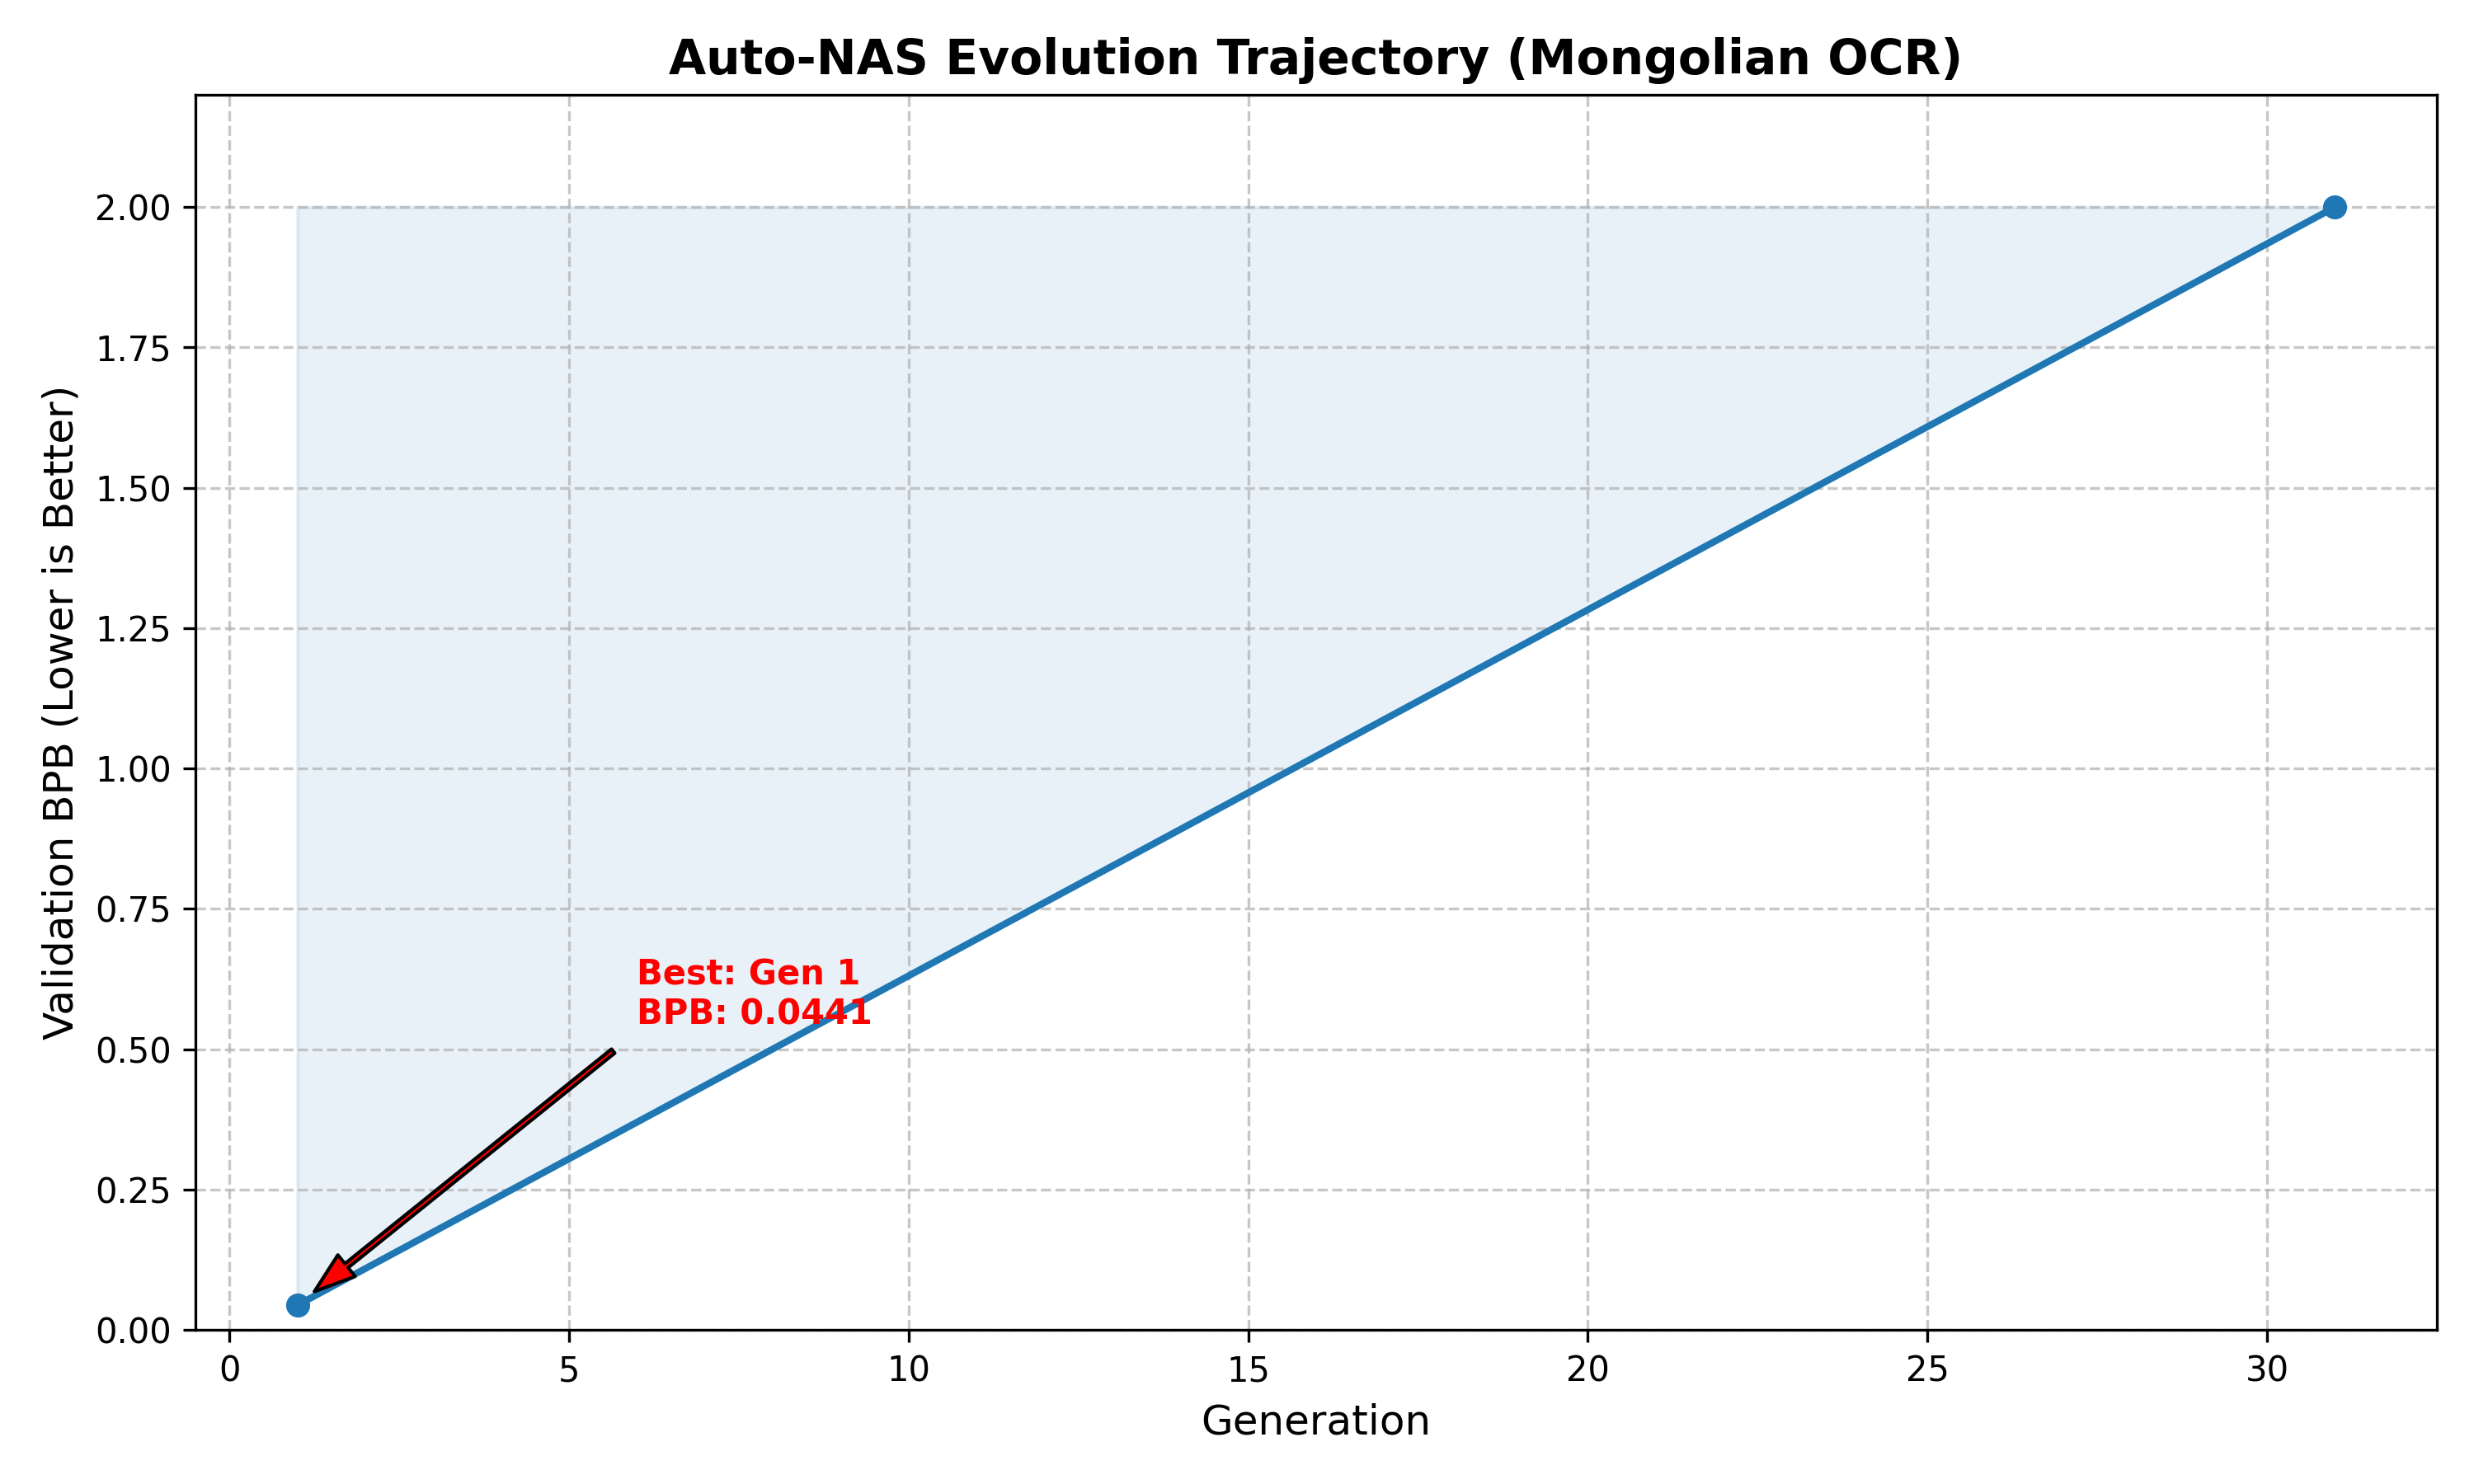
\includegraphics[width=0.82\textwidth]{figures/figure2_trajectory.png}
  \caption{The evolutionary search trajectory guided by the LLM over generations, demonstrating fitness convergence and the rejection of sub-optimal architectural mutations.}
  \label{fig:trajectory}
\end{figure*}

\subsection{Joint Optimization Objective}

The model is optimized with a joint loss
\begin{equation}
\mathcal{L} = \lambda_{\mathrm{det}}\mathcal{L}_{\mathrm{det}} + \lambda_{\mathrm{rec}}\mathcal{L}_{\mathrm{rec}},
\end{equation}
where $\mathcal{L}_{\mathrm{det}}$ denotes the detection loss and $\mathcal{L}_{\mathrm{rec}}$ denotes the CTC-based recognition loss. During architecture search, candidate acceptance is determined by a weighted fitness function
\begin{equation}
F = \alpha F_{\mathrm{det}} + \beta H_{\mathrm{e2e}},
\end{equation}
where $F_{\mathrm{det}}$ is the detection Hmean and $H_{\mathrm{e2e}}$ is the end-to-end spotting Hmean. To prioritize recognition-aware architectures, we set $\alpha = 0.3$ and $\beta = 0.7$ throughout search and final evaluation.

\subsection{Characteristics of the Searched Architecture}

The accepted architectures consistently display stronger directional sensitivity and tighter coupling between detection and recognition. Representative retained modules include AsymConvBlock, VerticalTPSLite, VerticalBiTrackAttention, and strip-pooling operations that increase vertical context aggregation without a large parameter overhead.

\begin{figure*}[t]
  \centering
  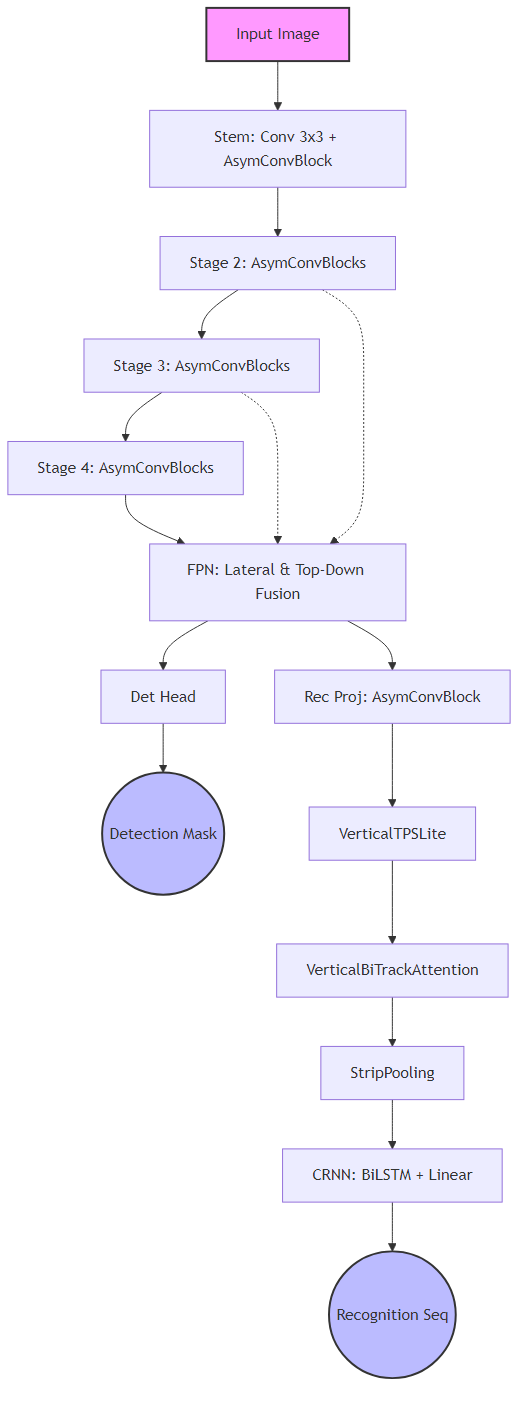
\includegraphics[height=0.72\textheight]{figures/figure3_architecture.png}
  \caption{The final searched joint architecture, highlighting directional feature extraction, region alignment, and decoupled spatial attention mechanisms.}
\end{figure*}

\section{Experimental Setup}

\subsection{Datasets}

We evaluate AutoArchival on two public end-to-end text spotting benchmarks and one target-domain historical benchmark.

\textbf{ICDAR 2015 (IC15).} IC15 is a standard benchmark for multi-oriented text spotting in natural scenes, containing 1,000 training images and 500 test images.

\textbf{Total-Text.} Total-Text contains 1,555 images with arbitrary-shaped and curved text, which stresses the robustness of region representations beyond straight bounding boxes.

\textbf{MCAD.} The Mongolian-Chinese Historical Archive Dataset contains 2,000 curated scans of eighteenth- and nineteenth-century archival documents, split into 1,500 training images and 500 test images. MCAD includes line-level polygon annotations and text transcriptions, covering dense vertical columns, bilingual layouts, overlapping red seals, and heavily degraded backgrounds. The annotation vocabulary contains 5,432 tokens, and all labels were manually cross-checked by two linguistic experts.

\subsection{Implementation Details}

All models are implemented in PyTorch and trained on a workstation with four NVIDIA RTX 3090 GPUs. We use AdamW with an initial learning rate of $10^{-4}$, weight decay $0.05$, and batch size 16. Final discovered models are trained from scratch for 100 epochs without external pretraining. Recognition decoding uses greedy CTC decoding without a language model.

\subsection{Evaluation Metrics}

We report detection, recognition, and end-to-end spotting metrics separately. Detection quality is measured by Hmean at an intersection-over-union threshold of 0.5. Recognition is measured by word accuracy on ICDAR 2015 and Total-Text, and by normalized edit distance (NED, reported as a percentage) on MCAD, where partial transcription quality is informative for agglutinative Mongolian sequences. End-to-end performance is reported with spotting Hmean, which counts a prediction as correct only when both localization and transcription are correct.

\section{Results and Discussion}

\subsection{Comparison with State-of-the-Art Methods}

Table~\ref{tab:public} compares AutoArchival with representative text spotting systems on ICDAR 2015 and Total-Text. AutoArchival achieves an end-to-end Hmean of 75.3\% on IC15 and 76.1\% on Total-Text. It outperforms classical baselines such as FOTS and Mask TextSpotter v3, remains competitive with stronger recent models, and uses only 14.5M parameters. These results indicate that LLM-guided code-level evolution can discover efficient detector-recognizer coupling patterns rather than simply scaling model size.

\begin{table*}[t]
\caption{Spotting performance on ICDAR 2015 and Total-Text. ``--'' indicates that standalone recognition metrics were not reported by the original authors under the protocol used here.}
\label{tab:public}
\centering
\resizebox{\textwidth}{!}{%
\begin{tabular}{lcccccc}
\toprule
Method & Params & IC15 Det & IC15 Rec & IC15 E2E & TT Rec & TT E2E \\
& & (Hmean) & (W.A.) & (Hmean) & (W.A.) & (Hmean) \\
\midrule
FOTS~\cite{liu2018fots} & $\sim$35M & 88.0 & 70.1 & 50.8 & 72.4 & 52.3 \\
Mask TextSpotter v3~\cite{liao2020mask} & $\sim$58M & 88.6 & 76.5 & 71.2 & 79.1 & 71.2 \\
ABCNet v2~\cite{liu2021abcnet} & $\sim$35M & 90.4 & -- & 73.8 & -- & 74.1 \\
DeepSolo~\cite{ye2023deepsolo} & $\sim$41M & 91.5 & -- & 77.2 & -- & 78.4 \\
Baseline seed & 24.5M & 84.2 & 65.4 & 60.1 & 66.8 & 58.9 \\
AutoArchival (ours) & 14.5M & 89.1 & 79.5 & 75.3 & 81.3 & 76.1 \\
\bottomrule
\end{tabular}}
\end{table*}

\subsection{Results on MCAD}

MCAD is the primary target domain for the proposed framework. As shown in Table~\ref{tab:mcad}, AutoArchival achieves 88.9\% detection Hmean, 89.2\% recognition NED, and 76.8\% end-to-end Hmean, outperforming all retrained baselines. The magnitude of improvement is larger on MCAD than on the public benchmarks, which supports the hypothesis that domain-specific architectural adaptation matters most when text geometry is strongly vertical and background degradation is severe.

\begin{table}[t]
\caption{Spotting performance on the MCAD benchmark.}
\label{tab:mcad}
\centering
\begin{tabular}{lccc}
\toprule
Method & Det & Rec & E2E \\
& (Hmean) & (NED) & (Hmean) \\
\midrule
FOTS (retrained) & 78.4 & 74.2 & 60.5 \\
Mask TextSpotter v3 (retrained) & 81.2 & 78.5 & 64.2 \\
ABCNet v2 (retrained) & 83.5 & 80.1 & 67.8 \\
AutoArchival (ours) & 88.9 & 89.2 & 76.8 \\
\bottomrule
\end{tabular}
\end{table}

The qualitative behavior of the searched modules is consistent with the quantitative gains. VerticalBiTrackAttention helps the recognizer preserve long top-to-bottom stroke continuity, while asymmetric convolution and vertical alignment reduce fragmentation in elongated text regions. These gains are less pronounced on public benchmarks because those datasets are dominated by horizontal or slightly curved text, where symmetric receptive fields are already effective.

\subsection{Ablation Study}

To isolate the contribution of the discovered modules, we replace the baseline components incrementally with AsymConvBlock, VerticalTPSLite, and VerticalBiTrackAttention. Table~\ref{tab:ablation} shows that asymmetric convolution alone raises end-to-end Hmean from 60.1\% to 66.5\%. Adding the lightweight vertical TPS alignment further improves localization and recognition, while the full combination yields the strongest result on all three MCAD metrics.

\begin{table}[t]
\caption{Ablation study of autonomously discovered modules on MCAD.}
\label{tab:ablation}
\centering
\begin{tabular}{cccccc}
\toprule
AsymConv & TPSLite & BiTrack & Det & Rec & E2E \\
& & & (Hmean) & (NED) & (Hmean) \\
\midrule
No & No & No & 82.1 & 72.3 & 60.1 \\
Yes & No & No & 85.3 & 75.8 & 66.5 \\
Yes & Yes & No & 86.8 & 79.1 & 71.0 \\
Yes & Yes & Yes & 88.9 & 89.2 & 76.8 \\
\bottomrule
\end{tabular}
\end{table}

\subsection{Efficiency Analysis}

AutoArchival is designed to search under a strict resource budget and therefore produces a compact final model. The discovered network runs at 22 FPS on a single RTX 3090 with batch size 1 at $1000 \times 1000$ input resolution and uses 1.2 GB peak inference memory. By contrast, heavier transformer-based spotters such as DeepSolo require substantially larger memory footprints. This makes AutoArchival attractive for practical archival digitization scenarios where throughput and deployment cost matter.

\subsection{Qualitative Results and Failure Cases}

Figure~\ref{fig:qualitative} summarizes typical qualitative outcomes. Compared with the baseline, AutoArchival better preserves long vertical text chains and reduces truncation in densely packed columns. The remaining failure cases are mainly detection-driven: when torn page boundaries or severe degradation intersect with the text line, the detector may truncate the proposal before the recognizer receives the full sequence. Ambiguous dialectal Mongolian variants can also confuse the CTC decoder. These observations suggest that future work should further strengthen proposal robustness and semantic post-correction.

\begin{figure*}[t]
  \centering
  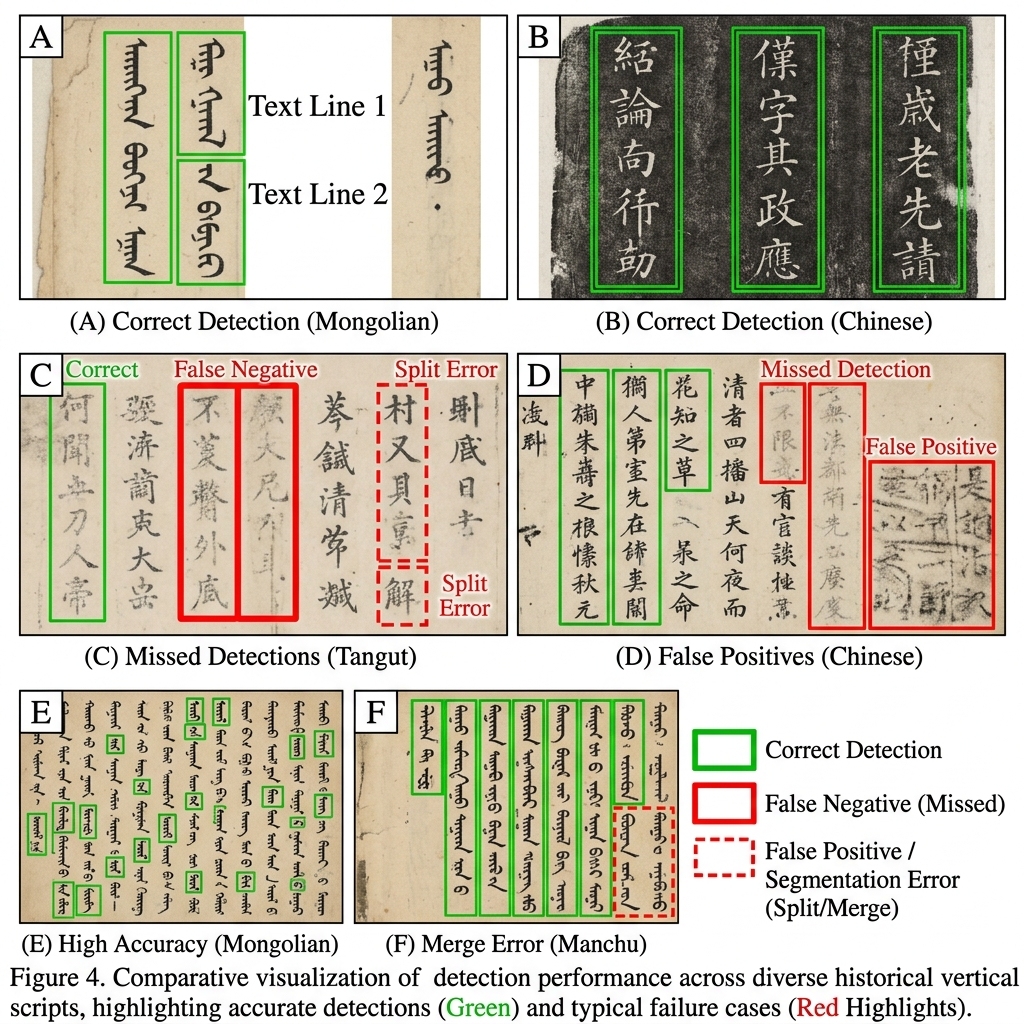
\includegraphics[width=0.95\textwidth]{figures/figure4_qualitative.png}
  \caption{Qualitative comparisons and representative failure cases on public benchmarks and MCAD. AutoArchival effectively localizes and decodes complex vertical structures.}
  \label{fig:qualitative}
\end{figure*}

\section{Conclusion}

We presented AutoArchival, a budget-constrained LLM-guided code-level architecture search framework for historical document text spotting. By searching editable detector-recognizer components under a fixed computational budget, the framework discovers directional modules that are well matched to degraded vertical Mongolian-Chinese archives. The resulting model improves substantially over the manually designed seed baseline, generalizes competitively to public benchmarks, and maintains a strong efficiency-performance trade-off. These findings suggest that constrained LLM-guided architecture search is a practical way to adapt end-to-end spotting systems to structurally specialized document domains.

\section*{Funding}

This work was supported by the National Natural Science Foundation of China (Grant No. 62341604), the Science and Technology Project of Inner Mongolia Autonomous Region Archives Bureau (Grant No. 2022-36), the China Scholarship Council (Grant No. 202408150080), and the General Project of the 14th Five-Year Plan for Educational Science of Inner Mongolia Autonomous Region (Grant No. NGJGH2025013).

\section*{Data Availability}

Public benchmark datasets used in this study are available from their original sources. The Mongolian-Chinese Historical Archive Dataset (MCAD), together with annotations, code, model configurations, and experiment scripts for AutoArchival, will be publicly released at \url{https://github.com/liuyuefeng/AutoArchival} upon acceptance of this paper.

\section*{Declaration of Competing Interest}

The authors declare that they have no known competing financial interests or personal relationships that could have appeared to influence the work reported in this paper.

\section*{Declaration of Generative AI in Scientific Writing}

Generative AI technologies (Claude and Gemini) were used solely for manuscript formatting and grammatical polishing.

\section*{Acknowledgements}

The authors thank the Inner Mongolia Autonomous Region Archives Bureau for its support.

\printcredits

\bibliographystyle{unsrtnat}
\bibliography{refs}

\end{document}
